\title{Survivability in slasher movies: \\abstinence and gender}
\author{Pedro Henrique Luz de Araujo}
\date{\today}

\documentclass[12pt]{article}
\usepackage{graphicx}
\usepackage{booktabs}
\usepackage{tabularx}
\usepackage{amsmath}

\begin{document}
\maketitle

\begin{abstract}
This is the paper's abstract \ldots
\end{abstract}

\section{Introduction}
Problem: Does gender influence survivability in slasher movies? Does sexual activity? How do they interact?

\paragraph{Outline}
The remainder of this article is organized as follows.
Section~\ref{previous work} gives account of previous work.
Our new and exciting results are described in Section~\ref{results}.
Finally, Section~\ref{conclusions} gives the conclusions.

\section{Data}\label{data}
The data\footnote{Welsh, A. On the Perils of Living Dangerously in the Slasher Horror Film: Gender Differences in the Association Between Sexual Activity and Survival. Sex Roles 62, 762–773 (2010). https://doi.org/10.1007/s11199-010-9762-x} include the survival status of 485 characters from 50 North American slasher films released between 1960 and 2009 randomly sampled from the Internet Movie Database (IMDb)\footnote{https://www.imdb.com/.}. The population was selected using keywords associated with the slasher genre; i.e.\ slasher, masked killer, gore, among others.

As explanatory variables we have the ``Gender'' and ``Involvement in Sexual Activity''. The first is taken to be the biological sex of the character, while the second is true if the character is involved with full or partial nudity or extended physical intimacy with another character. Only characters that suffered some kind of physical aggression are included. This was measured by undergraduate students. Refer to the original paper for a more detailed explanation of the data acquisition process.

Of all characters in the dataset, only 17.53\% survives. The survival rate is higher for women (22.52\%) than for men(13.30\%). In addition, despite women being the minority of cases (45.77\%), 52.87\% of characters involved in sexual activity are women. Table~\ref{tab:sexXgender} summarises the relation between gender and sexual activity. Figure~\ref{fig:pairs} exhibits the relationships between all variables. Note that characters that exhibit sexual activity are very unlikely to survive.

\begin{table}[hbtp]
    \centering
    \footnotesize
    \caption{Sexual activity across genders.}
    \label{tab:sexXgender}
    \begin{tabularx}{\textwidth}{X X X r}
        \toprule
        & \multicolumn{2}{c}{Gender} & Total \\
        \cmidrule{2-3}
        & Male & Female & \\
        \midrule 
        Presence & 74 & 83 & 157 \\
        Absence & 189 & 139 & 328\\  
        Total & 263 & 222& 485\\  
        \bottomrule
       \end{tabularx}
\end{table}



\begin{figure}[hbtp]  
    \centering
    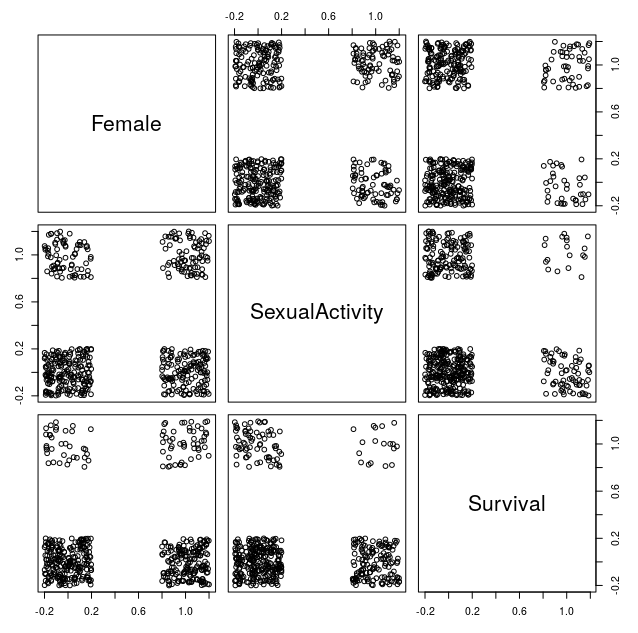
\includegraphics[width=0.5\textwidth]{media/pairs.png}
    \caption{Relationships between variables. Values have been jiggles, since all of them only assume 0 or 1 values.}
    \label{fig:pairs}
    \end{figure}

\section{Model}
Since we have a binary response variable, a logistic regression method is appropriate. We model the survival of character $i$, $y_i$, as a Bernoulli distribution with parameter $p_i$. Each $p_i$ is in turn, a function of the explanatory variables---Gender and Involvement in Sexual Activity---and learnable $\beta$ parameters. We add an interaction variable that is the product of Gender and Involvement in Sexual Activity in order to directly measure the interaction between such variables. Thus, the model has the following specification:
\begin{align}
    y_i | p_i &\stackrel{ind}{\sim} \text{Bern}(p_i),~i=1,\dots,n\\
    p_i &= \frac{1}{1+\text{exp}\left[-\left(\beta_0 + \beta_1G_i + \beta_2S_i + \beta_3\text{int}_i\right)\right]}\,,
\end{align}
where $G_1$, $S_i$ and $int_i$ are the Gender, Involvement in Sexual Activity and interaction variables of character $i$, respectively. Since the beta parameters give us a measure of how much each explanatory variable affects expectation of survival, this model allow us to answer the research questions.

As priors for the beta coefficients we chose a normal prior with mean 0 and variance 25. This prior is fairly noninformative for logistic regression, due to the sigmoid function. A noninformative prior is chosen to reflect our lack of strong a priori beliefs.

We fit the model using RJAGS. We establish fit 3 chains for 6000 iterations, filtering out the first 1000 as the burn-in period. This seemed to be sufficient for convergence (potential scale reduction factors of 1 for all parameters, and autocorrelation approaching zero).

\section{Results}\label{results}
In this section we describe the results.

\section{Conclusions}\label{conclusions}
We worked hard, and achieved very little.

\end{document}